\section{Widerstände}
	\begin{align*}
		R&=\varrho\cdot\frac{l}{A} &
		R&=\frac{U}{I} &
		r&=\frac{\mathrm{d}U}{\mathrm{d}I} &
		P&=U\cdot I=\frac{U^2}{R}=I^2\cdot R
	\end{align*}

	\begin{table}[h]
	\begin{tabular}{ll}
	$\varrho \left[\Omega\mathrm{cm}\equiv\Omega\frac{\mathrm{mm}^2}{\mathrm{m}}\right]\dots$ Spezifischer Widerstand & $l\dots$ Leitungslänge\\
	$r\dots$ dynamischer Widerstand(differenzieller Widerstand) & $A\dots$ Leitungsquerschnitt \\
	\end{tabular}
	\end{table}
		
	\subsection{Vernachlässigungsregeln}
		\begin{table}[here]
		\begin{tabular}{ll}
		Schaltungsart & Vernachlässigung\\
		\toprule
		Parallelschaltung & größerer Widerstand\\
		\midrule
		Reihenschaltung & kleinerer Widerstand\\
		\end{tabular}
		\end{table}

		Daumenregel: Ist ein Widerstand um den Faktor 10 größer als der andere kann man obige Regeln anwenden.
		Hilft auch bei kaskadiertem Spannungsteiler.

	\subsection{Temperaturabhängigkeit des Widerstands}
		\[
			R(\vartheta)=R_{20}\cdot\left[1+\alpha_{20}\cdot(\vartheta-20^{\circ}\mathrm{C})
			+\beta_{20}\cdot(\vartheta-20^{\circ}\mathrm{C})^2\right]
		\]

		\begin{table}[h]
		\begin{tabular}{ll}
		$\alpha\dots$ Temperaturkoeff. bei Raumtemperatur & $\beta\dots$ quadr. Temp.Koeff., meist vernachlässigbar\\
		\end{tabular}
		\end{table}

	\subsection{Erwärmung eines Bauteils}
		\[
			\vartheta_{\mathrm{E}}=P\cdot R_{\mathrm{th}}+\vartheta_{\mathrm{U}}
		\]

		\begin{table}[h]
		\begin{tabular}{ll}
		$R_{\mathrm{th}}\dots$ Wärmewiderstand in K/W & $C_{\mathrm{th}}\dots$ Wärmekapazität in Ws/K\\
		$\vartheta_{\mathrm{E}}\dots$ Endtemperatur & $\vartheta_{\mathrm{U}}\dots$ Umgebungstemperatur\\
		\end{tabular}
		\end{table}

	\subsection{Innenwiderstand und Überlagerungssatz}
		\subsubsection{Berechnung des Innenwiderstands}
			\begin{itemize}
				\item Betrachtung von den Anschlussklemmen des Lastwiderstands aus
				\item Ausschalten aller Quellen
				\item Innenwiderstand: Addition aller Widerstände nach o.g. Regeln \textbf{oder} $R=\frac{U_{\mathrm{L}}}{I_{\mathrm{K}}}$
				\item Leerlaufspannung ($U_{\mathrm{L}}$): Last ist abgeklemmt, Klemmen sind offen
				\item Kurzschlussstrom ($I_{\mathrm{K}}$): Last ist durch Draht überbrückt
			\end{itemize}
			\begin{table}[here]
			\begin{tabular}{ll}
			Quellenart & Stilllegung durch\\
			\toprule
			Stromquelle & Klemmen öffnen\\
			\midrule
			Spannungsquelle & kurzschließen\\
			\end{tabular}
			\end{table}

	\subsection{Nichtlineare Widerstände}
		\subsubsection{Abhängigkeiten}
			\begin{table}[here]
			\begin{tabular}{ll}
			Widerstand & Abhängigkeit\\
			\toprule
			Kaltleiter (PTC-Widerstand) & Temperatur steigt $\rightarrow$ Widerstand nimmt zu\\
			\midrule
			Heißleiter (NTC-Widerstand) & Temperatur steigt $\rightarrow$ Widerstand nimmt ab\\
			\midrule
			Varistor & Spannung steigt $\rightarrow$ Widerstand nimmt ab\\
			\end{tabular}
			\end{table}
\section{Kondensatoren}
	\subsection{Kapazität}
		\begin{align*}
			Q&=C\cdot U & i(t)&=\frac{\mathrm{d}Q}{\mathrm{d}t}=C\cdot\frac{\mathrm{d}u(t)}{\mathrm{d}t} & u(t)&=\frac{1}{C}\int i(t)\mathrm{d}t
		\end{align*}
	\subsection{Kondensator als Energiespeicher}
		\[
			W=\frac{1}{2}C\cdot u^2
		\]
	
	\subsection{RC-Netzwerke}

%		\begin{figure}[ht]
%			\begin{subfigure}{0.5\textwidth}
%			\begin{center}
%			\begin{circuitikz}
%			\draw
%			(0,0)node(gnd) {}
%			(0,2)node(R){}
%			(2,2)node(Co){}
%			(2,0)node(Cu){}
%			(3,2)node(Uo){}
%			(3,0)node(Uu){}
%			(R) to [R=$R$, o-*] (Co)
%			to [C=$C$,*-*] (Cu)
%			to [short, *-o] (gnd)
%			(Cu) to [short, *-o] (Uu)
%			(Co) to [short, *-o] (Uo)
%			(R) to [open, v>=$U_{\mathrm{e}}$] (gnd)
%			(Uu) to [open, v=$U_{\mathrm{a}}$] (Uo)
%			;
%			\end{circuitikz}
%			%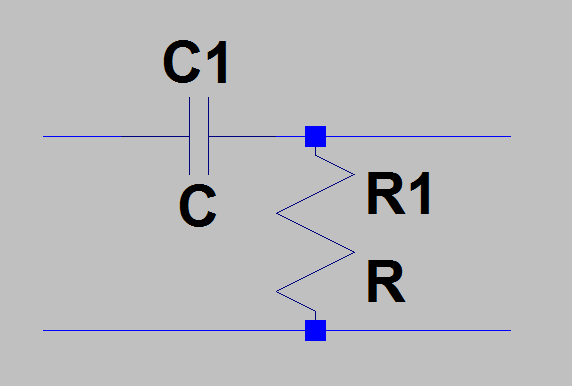
\includegraphics[width=\textwidth]{images/hochpass}
%			\end{center}
%			\caption{Hochpass}
%			\end{subfigure}
%			\begin{subfigure}{0.5\textwidth}
%			\begin{center}
%			\begin{circuitikz}
%			\draw
%			(0,0)node(gnd) {}
%			(0,2)node(C){}
%			(2,2)node(Ro){}
%			(2,0)node(Ru){}
%			(3,2)node(Uo){}
%			(3,0)node(Uu){}
%			(C) to [R=$R$, o-*] (Ro)
%			to [C=$C$,*-*] (Ru)
%			to [short, *-o] (gnd)
%			(Cu) to [short, *-o] (Uu)
%			(Co) to [short, *-o] (Uo)
%			(R) to [open, v>=$U_{\mathrm{e}}$] (gnd)
%			(Uu) to [open, v=$U_{\mathrm{a}}$] (Uo)
%			;
%			\end{circuitikz}
%			%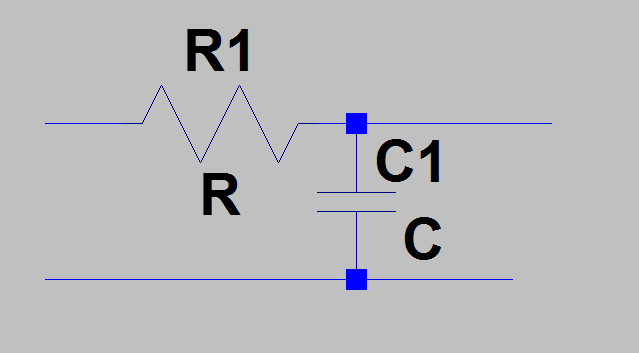
\includegraphics[width=\textwidth]{images/tiefpass}
%			\end{center}
%			\caption{Tiefpass}
%			\end{subfigure}
%		\end{figure}
		\begin{figure}[h]
		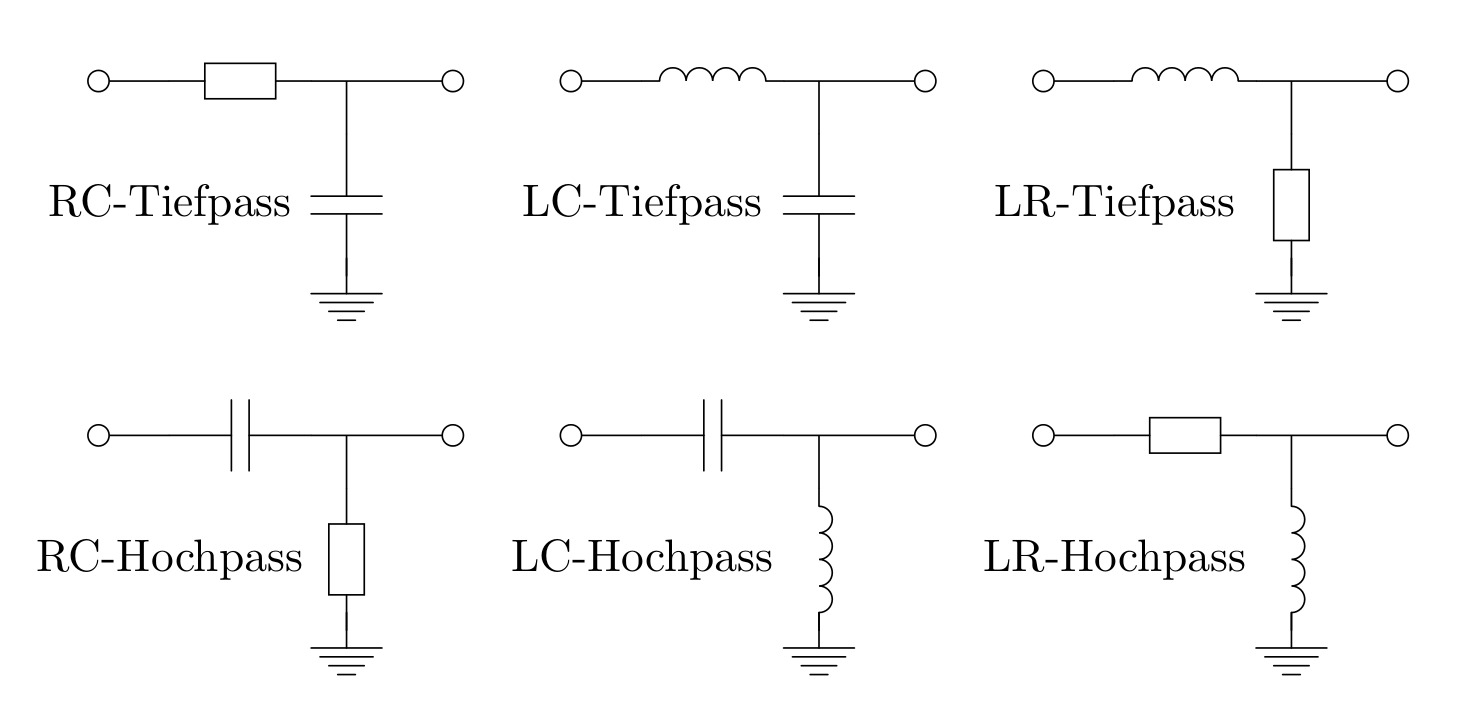
\includegraphics[width=\textwidth]{images/TP-HP-USW.png}
		\caption{Diverse Pässe}
		\end{figure}

		\subsubsection{Übertragungsfunktion}
			\begin{table}[h]
			\begin{tabular}{ll}
				Hochpass & Tiefpass\\
				\toprule
				$A_{\mathrm{HP}}=\frac{j\omega RC}{1+j\omega RC}$ & $A_{\mathrm{TP}}=\frac{1}{1+j\omega RC}$\\
				\midrule
				$\left|A\right|=\frac{\omega RC}{\sqrt{1+(\omega RC)^2}}$ & $\left|A\right|=\frac{1}{\sqrt{1+(\omega RC)^2}}$\\
				\midrule
				$\varphi=\arctan\left(\frac{1}{\omega RC}\right)$ & $\varphi=-\arctan\omega RC$\\
				\midrule
				$\omega_{\mathrm{G}}=\frac{1}{RC}$ & $\omega_{\mathrm{G}}=\frac{1}{RC}$\\
			\end{tabular}
			\end{table}
	\clearpage

	\section{Kondensator und Spule}
		\begin{table}[here]
		\begin{tabular}{lll}
		& Kondensator & Spule\\
		\toprule
		Allgemeine Formel & $(Y(0)-Y(\infty))\cdot e^{-\frac{t}{\tau}}+Y(\infty)$ & \\
		\midrule
		Ladung & $U_{\mathrm{C}}=U\left(1-e^{-\frac{t}{\tau}}\right)$ & $I_{\mathrm{L}}=\frac{U}{R}\left(1-e^{-\frac{t}{\tau}}\right)$\\
		\midrule
		Entladung & $U_{\mathrm{C}}=Ue^{-\frac{t}{\tau}}$ & $I_{\mathrm{L}}=I_0e^{-\frac{t}{\tau}}$\\
		\midrule
		Zeitkonstante & $\tau=RC$ & $\tau=\frac{R}{L}$\\
		\midrule
		Reduziert & Spannungsspitzen & Stromspitzen\\
		\end{tabular}
		\end{table}	
